%%%%%%%%%%%%%%%%%%%%%%%% ExtendedAbstract.tex %%%%%%%%%%%%%%%%%%%%%%%%
%                                                                    %
%  Template for the 10-page extended abstract to be submitted for    %
%  the MSc degree conferral at Instituto Superior Tecnico.           %
%                                                                    %
%  Author:                                                           %
%                                                                    %
%       Andre C. Marta                                               %
%       Area Cientifica de Mecanica Aplicada e Aeroespacial          %
%       Departamento de Engenharia Mecanica                          %
%       Instituto Superior Tecnico                                   %
%       Av. Rovisco Pais                                             %
%       1049-001 Lisboa                                              %
%       Portugal                                                     %
%       Tel: +351 21 841 9466                                        %
%                        3466 (extension)                            %
%       Email: andre.marta@ist.utl.pt                                %
%                                                                    %
%  Created:       Dec  2, 2011                                       %
%  Last Modified: Dec 27, 2011                                       %
%%%%%%%%%%%%%%%%%%%%%%%%%%%%%%%%%%%%%%%%%%%%%%%%%%%%%%%%%%%%%%%%%%%%%%
% This document uses the LaTeX class file "article.cls"              %
%%%%%%%%%%%%%%%%%%%%%%%%%%%%%%%%%%%%%%%%%%%%%%%%%%%%%%%%%%%%%%%%%%%%%%
\documentclass[10pt,a4paper,twocolumn,number]{article}

%%%%%%%%%%%%%%%%%%%%%%%%%%%%%%%%%%%%%%%%%%%%%%%%%%%%%%%%%%%%%%%%%%%%%%
% Document preamble
%%%%%%%%%%%%%%%%%%%%%%%%%%%%%%%%%%%%%%%%%%%%%%%%%%%%%%%%%%%%%%%%%%%%%%
\usepackage[utf8]{inputenc}
\usepackage[english]{babel}
\usepackage{caption}
\usepackage[table,xcdraw]{xcolor}
\usepackage{multirow}
\usepackage{hhline}
\usepackage{booktabs}
\usepackage{tikz}
\usepackage[compat=1.1.0]{tikz-feynman}
\usepackage{graphicx}
%% Builds upon the graphics  package, providing a key-value interface
%% for optional arguments to the \includegraphics command that go far
%% beyone what the graphics package offers.
%% http://www.ctan.org/tex-archive/help/Catalogue/entries/graphicx.html
%% if you use PostScript figures in your article
%% use the graphics package for simple commands
%% \usepackage{graphics}
%% or use the graphicx package for more complicated commands
%% \usepackage{graphicx}
%% or use the epsfig package if you prefer to use the old commands
%% \usepackage{epsfig}
\usepackage{graphicx} % Enhanced LaTeX Graphics

% Multiple figures
\usepackage{subfigure} % subcaptions for subfigures
\usepackage{subfigmat} % matrices of similar subfigures

% Declaring new column types
% 'dcolumn' package defines D to be a column specifier with
% three arguments: D{<sep.tex>}{<sep.dvi>}{<decimal places>}
%                  D{<sep.tex>}{<sep.dvi>}{<left digit places>.<right digit places>}
\usepackage{dcolumn}           % decimal-aligned tabular math columns
% d takes a single argument specifying the number of decimal places, e.g., d{2}
% or the number of digits to the left and right of the seperator, e.g., d{3.2}
\newcolumntype{.}   {D{.}{.}{-1}} % column alignedd on the point separator '.'
\newcolumntype{d}[1]{D{.}{.}{#1}} % column centered on the point separator '.'
\newcolumntype{e}   {D{E}{E}{-1}} % column centered on the exponent 'E'
\newcolumntype{E}[1]{D{E}{E}{#1}} % column centered on the exponent 'E'

%% American Mathematical Society (AMS) plain Tex macros
%%
%% The amsmath package is the principal package in the AMS-LaTeX distribution
%% http://www.ctan.org/tex-archive/help/Catalogue/entries/amsmath.html
\usepackage{amsmath}
%%
%% The amsfonts package provides extended TeX fonts
%% http://www.ctan.org/tex-archive/help/Catalogue/entries/amsfonts.html
\usepackage{amsfonts}
%% The amssymb package provides various useful mathematical symbols
\usepackage{amssymb}
%%
%% The amsthm package provides extended theorem environments
%% http://www.ctan.org/tex-archive/help/Catalogue/entries/amsthm.html
\usepackage{amsthm}

%% Improves the interface for defining floating objects such as figures and tables.
%% The package also provides the H float modifier option of the obsolete here package.
%% http://www.ctan.org/tex-archive/help/Catalogue/entries/float.html
\usepackage{float}

%% Control sectional headers. 
%% http://www.ctan.org/tex-archive/help/Catalogue/entries/sectsty.html
\usepackage{sectsty}
%%
%% Redefine the font size of the 'section' and 'subsection' headings
\newcommand{\myFontSize}{\fontsize{12}{0}\selectfont}
\sectionfont{\myFontSize}       % 10pt, Bold face (default)
\newcommand{\myFontSizeOi}{\fontsize{10}{0}\selectfont\bfseries}
\subsectionfont{\rm\myFontSizeOi} % 10pt, Plain face

%% Select alternative section titles.
%% http://www.ctan.org/tex-archive/help/Catalogue/entries/titlesec.html
\usepackage{titlesec}
\usepackage{etoolbox}

\makeatletter
\patchcmd{\ttlh@hang}{\parindent\z@}{\parindent\z@\leavevmode}{}{}
\patchcmd{\ttlh@hang}{\noindent}{}{}{}
\makeatother
%%
%% Left indent, before and after spacing
%% (The starred version kills the indentation of the paragraph following the title)
\titlespacing*{\section}{0pt}{10pt}{0pt}
\titlespacing*{\subsection}{0pt}{10pt}{0pt}

%% Section numbers with trailing dots. 
%% http://www.ctan.org/tex-archive/help/Catalogue/entries/secdot.html
\usepackage{secdot}
%%
%% Also put a dot after the subsection number
\sectiondot{subsection}
%% Set a space between dot and heading text
\sectionpunct{section}{. }    % By default, \sectiondot places a \quad
\sectionpunct{subsection}{. } % after the number

% These are exact settings for a A4 page with top margin of
% 25 mm, bottom margin of 30 mm, left and right margins of 25 mm,
% printable area 242 X 160 mm.

\setlength{\topmargin}{-10.4mm}
\setlength{\headheight}{0.0mm}
\setlength{\headsep}{10.0mm}
\setlength{\textwidth}{160mm}
\setlength{\textheight}{242mm}
\setlength{\oddsidemargin}{0mm}
\setlength{\evensidemargin}{0mm}
\setlength{\marginparwidth}{0mm}
\setlength{\marginparsep}{0mm}

% New command to refer to equations as Eq.(1),Eq.(2),...
\newcommand{\eqnref}[1]{Eq.(\ref{#1})}

%%%%%%%%%%%%%%%%%%%%%%%%%%%%%%%%%%%%%%%%%%%%%%%%%%%%%%%%%%%%%%%%%%%%%%%%%%%%%%%%%%%%%%%%
% Title, authors and addresses

\title{Higgs pair production in the four b quarks final state }
\date{December 2011}
\author{Ana Lu\'{i}sa Moreira de Carvalho \\ \\ Instituto Superior T\'{e}cnico, Lisboa, Portugal}

%%%%%%%%%%%%%%%%%%%%%%%%%%%%%%%%%%%%%%%%%%%%%%%%%%%%%%%%%%%%%%%%%%%%%%%%%%%%%%%%%%%%%%%%
\begin{document}

% Begin one column section for title and abstract
%
% http://www.faqs.org/faqs/de-tex-faq/part5/
\twocolumn[
\begin{@twocolumnfalse}
\maketitle

%%%%%%%%%%%%%%%%%%%%%%%%%%%%%%%%%%%%%%%%%%%%%%%%%%%%%%%%%%%%%%%%%%%%%%
% ABSTRACT & KEYWORDS
%%%%%%%%%%%%%%%%%%%%%%%%%%%%%%%%%%%%%%%%%%%%%%%%%%%%%%%%%%%%%%%%%%%%%%
%%%%%%%%%%%%%%%%%%%%%%%%%%%%%%%%%%%%%%%%%%%%%%%%%%%%%%%%%%%%%%%%%%%%%%
%     File: ExtendedAbstract_abstr.tex                               %
%     Tex Master: ExtendedAbstract.tex                               %
%                                                                    %
%     Author: Andre Calado Marta                                     %
%     Last modified : 2 Dez 2011                                     %
%%%%%%%%%%%%%%%%%%%%%%%%%%%%%%%%%%%%%%%%%%%%%%%%%%%%%%%%%%%%%%%%%%%%%%
% The abstract of should have less than 500 words.
% The keywords should be typed here (three to five keywords).
%%%%%%%%%%%%%%%%%%%%%%%%%%%%%%%%%%%%%%%%%%%%%%%%%%%%%%%%%%%%%%%%%%%%%%

%%
%% Abstract
%%
\begin{abstract}

This article presents a feasibility study targeting the search for Higgs pairs in the $hh\rightarrow b\overline{b}b\overline{b}$ channel at a center of mass energy of $\sqrt{s}=100$ TeV at a future hadronic circular collider, considering a high integrate luminosity. For Standard Model production of Higgs pairs, the achieved significance with a simple cut-based boosted analysis is $S/\sqrt{B}=8.8\pm 1.6~\text{(stat.)}~^{+4.4}_{-3.4}~\text{(sys.)}$. The change in the significance as a function of the granularity of the hadronic calorimeter is studied, targeting the optimization of the design of future detectors.
\\
%%
%% Keywords (max 5)
%%
\noindent{{\bf Keywords:}} Higgs pair production, Future Circular Collider, FCC-hh, four b quarks final state\\

\end{abstract}



% End one column section (begin default two columns)
\end{@twocolumnfalse}
]
%%%%%%%%%%%%%%%%%%%%%%%%%%%%%%%%%%%%%%%%%%%%%%%%%%%%%%%%%%%%%%%%%%%%%%
% INTRODUCTION
%%%%%%%%%%%%%%%%%%%%%%%%%%%%%%%%%%%%%%%%%%%%%%%%%%%%%%%%%%%%%%%%%%%%%%
%%%%%%%%%%%%%%%%%%%%%%%%%%%%%%%%%%%%%%%%%%%%%%%%%%%%%%%%%%%%%%%%%%%%%%
%     File: ExtendedAbstract_intro.tex                               %
%     Tex Master: ExtendedAbstract.tex                               %
%                                                                    %
%     Author: Andre Calado Marta                                     %
%     Last modified : 27 Dez 2011                                    %
%%%%%%%%%%%%%%%%%%%%%%%%%%%%%%%%%%%%%%%%%%%%%%%%%%%%%%%%%%%%%%%%%%%%%%
% State the objectives of the work and provide an adequate background,
% avoiding a detailed literature survey or a summary of the results.
%%%%%%%%%%%%%%%%%%%%%%%%%%%%%%%%%%%%%%%%%%%%%%%%%%%%%%%%%%%%%%%%%%%%%%

\section{Introduction and motivation}
\label{sec:intro}

%- Higgs pair production as a benchmark physics process for HL and future colliders (discovery inaccessible at the LHC)\\
%- Boosted analysis shows better sensitivity because QCD background can be kept under control \\
%- When using boosted jets we need to resolve their substructure (jet substructure observables)\\
%- The granularity of the (hadronic) calorimeter is a key parameter that determines how well we can resolve the substructure \\
%- The final state with four b quarks benefits from the largest BR and is a source of fully hadronic boosted Higgs jets \\
%- Goals of the work: estimate analysis sensitivity to Higgs trilinear coupling and study the influence of the HCAL granularity in the analysis \\

A lot of work is currently being put into designing and understanding the physics reach of future particle colliders. The hadronic Future Circular Collider (FCC-hh) study, led by CERN, is one of the possibilities that is currently being analyzed. Its baseline design consists of a $100$ km ring located in the Geneva area capable of delivering proton-proton collisions at a center of mass energy of $100$ TeV. The next milestone for this project is the delivery of a Conceptual Design Report (CDR) by the end of 2018. This document should include a first cost estimate as well as a compilation of preliminary analysis that illustrate the physics potential of such an accelerator.

A particularly interesting benchmark process to be studied in future colliders is the production of pairs of Higgs bosons (or di-Higgs production). This process is sensitive to the value of the Higgs boson triple coupling that determines the shape of the Higgs potential and therefore plays a crucial role in the electroweak symmetry breaking mechanism. The leading order Feynamn diagrams that contribute to Higgs pair production through gluon-gluon fusion are shown in figure \ref{fig:hh_diag}. The top diagram is the one that provides sensitivity to the triple coupling.

\begin{figure}[h]
	\centering
	\feynmandiagram [baseline=(current bounding box.center),small, horizontal=e to f] {
		a -- [gluon, edge label'=\(g\)] b -- [anti fermion] c -- [gluon, edge label'=\(g\)] d,
		b -- [fermion] e -- [fermion] c,
		e -- [scalar, edge label'=\(h^*\)]  f,
		h -- [scalar, edge label'=\(h\)] f -- [scalar, edge label'=\(h\)] i,
		a -- [opacity=0] d,
	};\\
	\feynmandiagram[baseline=(current bounding box.center),small, layered layout,horizontal=a to b] {
		% Draw the top and bottom lines
		i1 -- [gluon, edge label'=\(g\)] a-- [anti fermion] b-- [scalar, edge label'=\(h\)] f1,
		i2 -- [gluon, edge label'=\(g\)] c-- [fermion] d-- [scalar, edge label'=\(h\)] f2,
		% Draw the two internal fermion lines
		{ [  same layer	] a -- [fermion] c },
		{ [  same layer] b -- [anti fermion] d},
	};
	\caption{Feynman diagrams for the $gg\rightarrow hh$ process at leading order.}
	\label{fig:hh_diag}
\end{figure}

However, searches for di-Higgs production are extremely challenging mainly because the cross section of this process is very small, of the order of tens of femtobarns (fb). Even with the entire dataset that is expected to be accumulated during the LHC's and its high luminosity upgrade lifetime ($O(3)~\text{ab}^{-1}$), it is very unlikely that we will be able to declare the observation of this process. Therefore, the discovery of di-Higgs production relies on future colliders making it a key benchmark process.

In this work we focus on the final state with four b quarks. The $h\rightarrow b\overline{b}$ decay has the largest of all Higgs branching ratios (BR), approximately $58\%$. Therefore this final state maximizes the cross section times branching of the $hh\rightarrow b\overline{b}b\overline{b}$ process. However, for this final state, the dominant background is multijet production through quantum chromodynamics (QCD) processes whose cross section is a lot larger than that of the signal. Nonetheless, it is a well known characteristic of QCD interactions that the partons (and jets) produced tend to have a low transverse momentum ($p_T$). This indicates that exploring a high $p_T$ region of the phase space could be the key to suppress the QCD multijet background. Such region is called boosted due to the high Lorentz boost of the objects involved. In this kinematic regime, traditional jet reconstruction algorithms, that establish a one to one correspondence between the partons and the jets, begin to fail because the $\Delta R=\sqrt{(\Delta\phi)^2+(\Delta\eta)^2}$ distance between the b quarks, $\Delta R(b\overline{b})$, gets increasingly smaller as the $p_T$ of the mother Higgs boson, $p_T(h_1)$, increases. This is shown in figure \ref{fig:deltaRbb_pt}. State of the art jet reconstruction techniques \cite{jetsub} use a single jet with a large $R$ parameter to reconstruct both b quarks as a single jet that is used as a $\textit{proxy}$ for the Higgs boson. In order to extract as much information as possible from these jets it is important to analyze its intrinsic structure, referred to as substructure. Such techniques are fairly recent and usually explore the existence of localized energy maximums inside a large $R$ jet (subjets). For example, a jet that contains the two b quarks coming from the decay of a Higgs boson is expected to be more compatible with the existence of two subjets than a jet produced by a QCD process.

\begin{figure}[h]
	\centering
	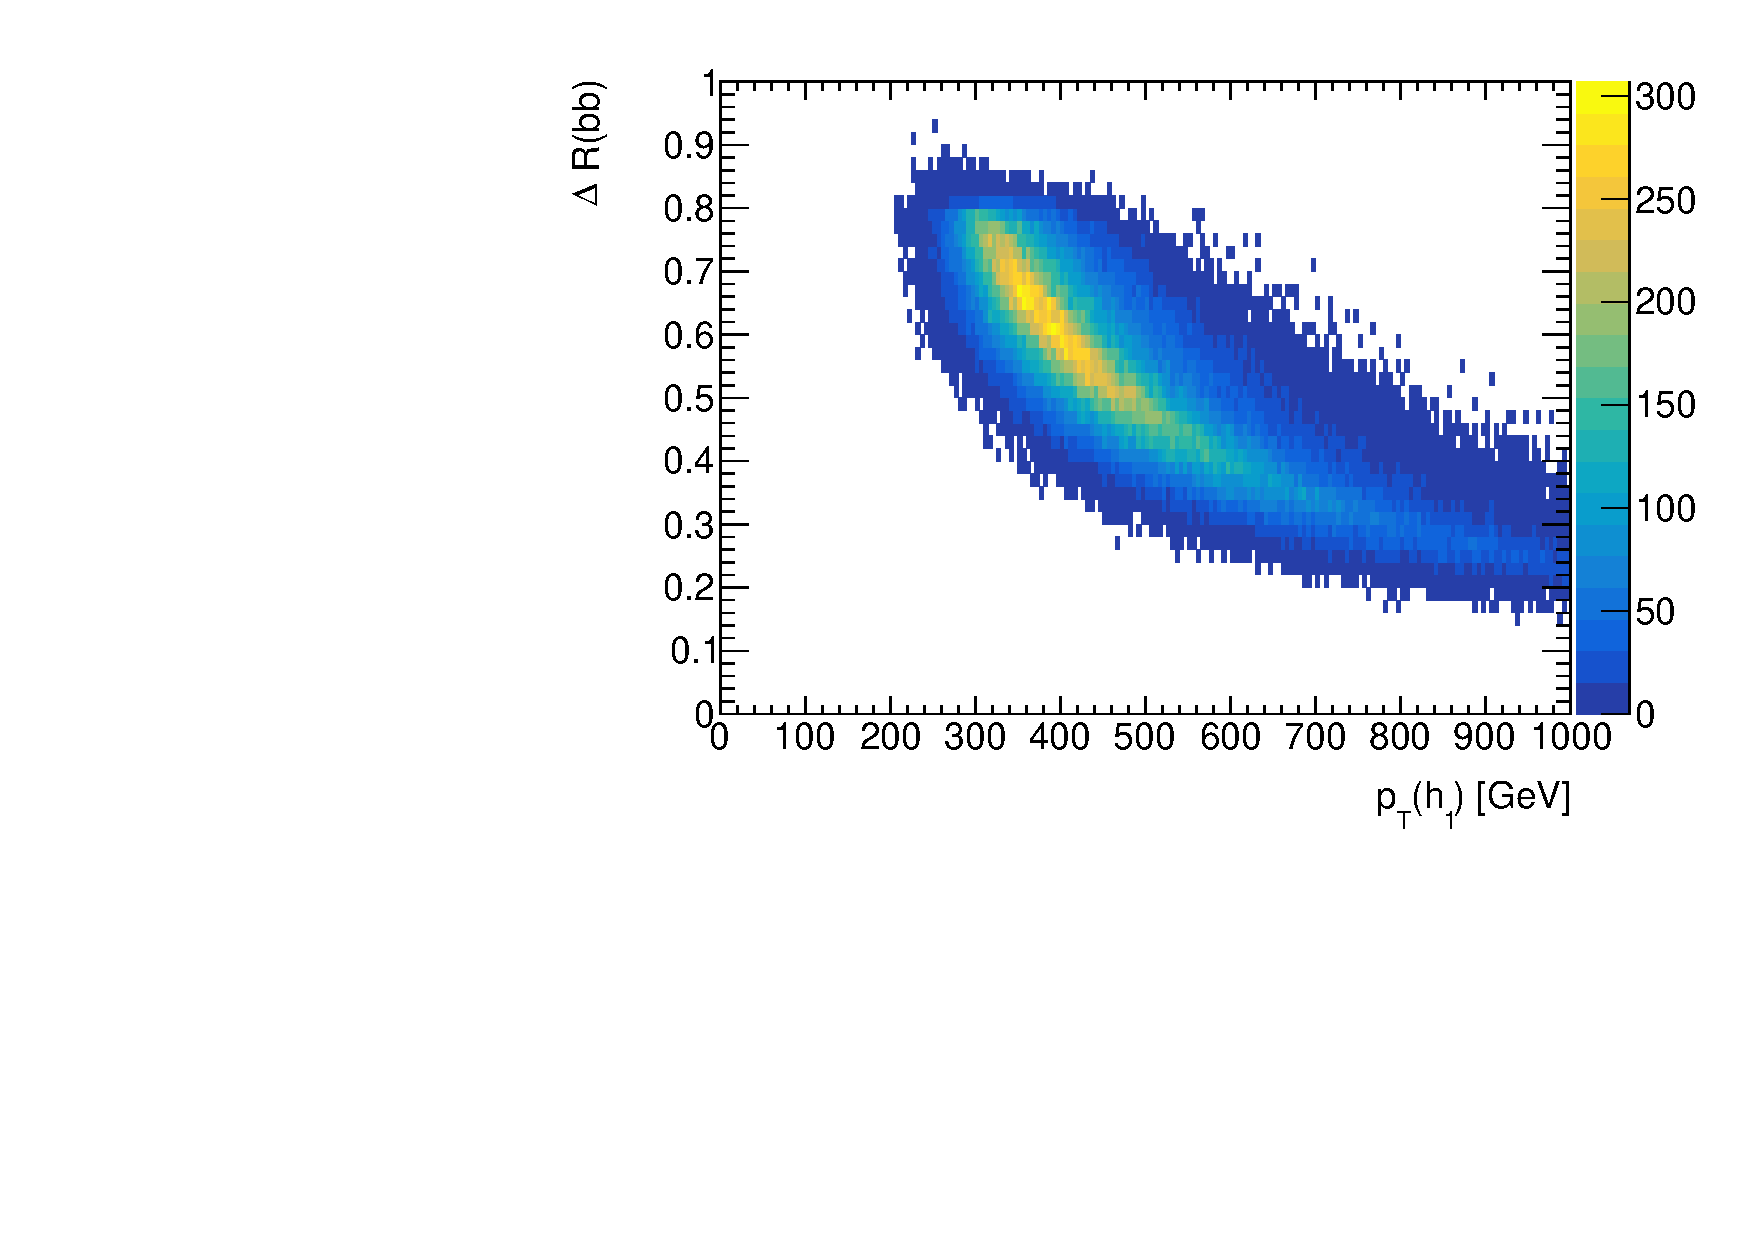
\includegraphics[trim={.5cm 0 0 0},clip,width=\linewidth]{./images/hist_deltaR_bb_pt.pdf}
	\caption{$\Delta R$ between the b quarks from the decya of the leading Higgs candidate as a function of its $p_T$.}
	\label{fig:deltaRbb_pt}
\end{figure}

From the point of view of detector design for the FCC-hh, as well as for future upgrades of existent detectors such as the ATLAS one, the granularity of the hadronic calorimeter (HCAL) is a key parameter because it greatly influences the ability of the detector to resolve the substructure of large $R$ jets. 

The main goal of this project is to use boosted di-Higgs production in the four b quarks final state to study the influence of the granularity of the HCAL in the significance ($S/\sqrt{B}$) that can be achieved.  



%%%%%%%%%%%%%%%%%%%%%%%%%%%%%%%%%%%%%%%%%%%%%%%%%%%%%%%%%%%%%%%%%%%%%%
%     File: ExtendedAbstract_imple.tex                               %
%     Tex Master: ExtendedAbstract.tex                               %
%                                                                    %
%     Author: Andre Calado Marta                                     %
%     Last modified : 27 Dez 2011                                    %
%%%%%%%%%%%%%%%%%%%%%%%%%%%%%%%%%%%%%%%%%%%%%%%%%%%%%%%%%%%%%%%%%%%%%%
% A Calculation section represents a practical development
% from a theoretical basis.
%%%%%%%%%%%%%%%%%%%%%%%%%%%%%%%%%%%%%%%%%%%%%%%%%%%%%%%%%%%%%%%%%%%%%%

\section{Collider experiments}
\label{sec:det}

\subsection{The LHC and the ATLAS detector}
 
The Large Hadron Collider (LHC) is housed by the European Organization for Nuclear Reasearch (CERN) and located beneath the Franco-Swiss boarder in the Geneva area. It consists of a $27$ km ring dedicated (most of the time) to delivering proton-proton collisions at a center of mass (CM) energy of $\sqrt{s}=13$ TeV. The two general purpose experiments, ATLAS and CMS, have a broad experimental physics program that includes searches for new physics. The LHCb experiment is dedicated to the study of beauty particles and the ALICE experiment is optimized to study heavy ion collisions. 

The ATLAS detector is a multipurpose particle physics apparatus with forward-backward symmetric  cylindrical geometry. A combination of cartesian and cylindrical coordinates is used to describe it. The origin is defined to coincide with the interaction point. The Cartesian system is right-handed and the z axis is defined to be the direction of the beam. The x-axis points from the interaction point to the center of the LHC ring and the y-axis points upwards. The azimuthal angle, $\phi$, is measured around the beam axis and the polar angle, $\theta$, from the beam line. The pseudorapidity is defined as $\eta = − \ln \tan(\theta/2)$. The inner tracking detector (ID) consists of  a  silicon  pixel detector,  a  silicon  microstrip detector, and a straw-tube transition radiation tracker. It is contained in a superconducting solenoid magnet that provides a $2$ T magnetic field and surrounded by a high-granularity liquid-argon sampling electromagnetic calorimeter (ECAL). The ECAL covers the pseudo-rapidity range $|\eta|<3.2$. The hadronic calorimetry in the pseudorapidity range $|\eta| < 1.7$ is provided by a scintillator-tile calorimeter (TileCal). For $|\eta|>1.5$ liquid-argon calorimeters extend the pseudorapidity range to $|\eta|=4.9$. The LAr calorimeter is divided in end-cap and forward. These cover the pseudorapidity ranges $1.5 < |\eta| < 3.2$ and $3.2 < |\eta| <
4.9$. In the end-cap the segmentation is $\Delta\eta\times\Delta\phi = 0.1 \times 0.1$ for $1.5 < |\eta| < 2.5$ and $0.2 \times 0.2$ for $2.5 < |\eta| < 3.2$. In the forward region the segmentation is $\Delta\eta\times\Delta\phi = 0.2 \times 0.2$. The muon spectrometer (MS) surrounds the calorimeters and it is the outermost layer of the detector. It is composed of Monitored Drift Tubes and Cathode Strip Chambers.

\subsection{The FCC-hh}

The FCC-hh baseline design consist of a of a proton-proton circular collider with a maximum CM energy of $\sqrt{s}=100$ TeV housed by a $100$ km tunnel in the area of Geneva. It will deliver a peak luminosity of $\mathcal{L}=30\times 10^{34}~\text{cm}^{-2}\text{s}^{-1}$ in its ultimate phase which will result in a $O(30)~\text{ab}^{-1}$ per experiment. This machine will extend the research program of the LHC (and of the HL-LHC) after these have reached their full discovery potential, by around 2040.

The design of the FCC-hh baseline detector has been greatly based on that of the ATLAS and CMS experiments, in particular the central barrel. The layers and sub detectors are arranged in the same order and make use of very similar technologies. The ID detector covers the pseudorapidity range $|\eta|<6$ and it will be instrumented with pixel and strip detectors. The ECAL covers the pseudorapidity range $|\eta|<6$. The proposed layout is a LAr sampling configuration with lead, glue and steal plates as absorbers. The granularity is expected to be two to four times better than for the ATLAS ECAL. The hadronic calorimeter covers the pseudorapidity range $|\eta| < 6$. It is divided in barrel, end-cap and forward that cover the pseudorapidity ranges $|\eta| < 1.3$, $1.0 < |\eta| < 1.8$ and $2.3 < |\eta| < 6.0$. For the barrel and end-cap calorimeters, the expected segmentation $\Delta\eta\times\Delta\phi = 0.025 \times 0.025$ while for the forward calorimeter it is $\Delta\eta\times\Delta\phi = 0.05 \times 0.05$. Overall, this corresponds to approximately four times the ATLAS HCAL granularity. The MS cover the pseudorapidity range $|\eta|<6$ and it consists of a layered structure of gas chambers.

%%%%%%%%%%%%%%%%%%%%%%%%%%%%%%%%%%%%%%%%%%%%%%%%%%%%%%%%%%%%%%%%%%%%%%%
%     File: ExtendedAbstract_imple.tex                               %
%     Tex Master: ExtendedAbstract.tex                               %
%                                                                    %
%     Author: Andre Calado Marta                                     %
%     Last modified : 27 Dez 2011                                    %
%%%%%%%%%%%%%%%%%%%%%%%%%%%%%%%%%%%%%%%%%%%%%%%%%%%%%%%%%%%%%%%%%%%%%%
% A Calculation section represents a practical development
% from a theoretical basis.
%%%%%%%%%%%%%%%%%%%%%%%%%%%%%%%%%%%%%%%%%%%%%%%%%%%%%%%%%%%%%%%%%%%%%%

\section{The FCC-hh and the baseline detector}
\label{sec:detFCC}
 

%%%%%%%%%%%%%%%%%%%%%%%%%%%%%%%%%%%%%%%%%%%%%%%%%%%%%%%%%%%%%%%%%%%%%%
% BACKGROUND
%%%%%%%%%%%%%%%%%%%%%%%%%%%%%%%%%%%%%%%%%%%%%%%%%%%%%%%%%%%%%%%%%%%%%%
%%%%%%%%%%%%%%%%%%%%%%%%%%%%%%%%%%%%%%%%%%%%%%%%%%%%%%%%%%%%%%%%%%%%%%
%     File: ExtendedAbstract_backg.tex                               %
%     Tex Master: ExtendedAbstract.tex                               %
%                                                                    %
%     Author: Andre Calado Marta                                     %
%     Last modified : 27 Dez 2011                                    %
%%%%%%%%%%%%%%%%%%%%%%%%%%%%%%%%%%%%%%%%%%%%%%%%%%%%%%%%%%%%%%%%%%%%%%
% A Theory section should extend, not repeat, the background to the
% article already dealt with in the Introduction and lay the
% foundation for further work.
%%%%%%%%%%%%%%%%%%%%%%%%%%%%%%%%%%%%%%%%%%%%%%%%%%%%%%%%%%%%%%%%%%%%%%

\section{State of the art}
\label{sec:backg}

%- HL upgrades for the LHC \\
%- FCC-hh, 100 TeV hadronic collider at the stage of CDR \\
%- Feasibility studies/previous work on this channel (slightly longer literature review)\\

The searches performed so far for di-Higgs production covered different decay channels and targeted not only the SM production but also some BSM scenarios where this process is enhanced. Neither could achieve enough statistical significance to declare the observation of this process nor found any deviation from the SM predictions. 

The most stringent limit comes from a combination of searches using up to $36.1~\text{fb}^{-1}$ of proton-proton collision data at a center of mass energy $\sqrt{s}=13$ TeV recorded with the ATLAS detector. The combination is performed using the analysis searching for $hh\rightarrow b\overline{b}b\overline{b}$, $hh\rightarrow b\overline{b}\tau^+\tau^.$ and $hh\rightarrow b\overline{b}\gamma\gamma$. The combined observed (expected) limit on the non-resonant Higgs boson pair cross-section is $0.22$ pb ($0.35$ pb) at $95\%$ confidence level, which corresponds to $6.7 (10.4)$ times the predicted SM cross-section. The ratio of the Higgs boson self-coupling to its SM expectation ($k_{\lambda}=\lambda_{hhh}/\lambda_{hhh}^{SM}$) is observed (expected) to be contrained at $95\%$ CL to $-5.0<k_{\lambda}<12.1 (-5.8<k_{\lambda}<12.0)$.

Monte Carlo studies assessing the feasibility of searches for di-Higgs production at the High Luminosity LHC (HL-LHC) and at the FCC-hh have been performed. For the HL-LHC, a study including the $pp\rightarrow b\overline{b}b\overline{b}$, $pp\rightarrow b\overline{b}jj$, $pp\rightarrow jjjj$ and $pp\rightarrow t\overline{t}jjjj$ reports a significance of $S/\sqrt{B}=3.1~(1.0)$ for an integrated luminosity of $3000~(300)~\text{fb}^{-1}$, considering a mean pileup of $80$. The analysis is performed in three orthogonal signal categories (resolved, intermediate and boosted) and the reported significance is obtained from the combination of the three regions. This study makes use of an artificial neural network to further increase the signal-background separation. Similar studies performed by ATLAS and CMS find the $hh\rightarrow b\overline{b}\gamma\gamma$ channel to be the most sensitive to the Higgs trilinear coupling. ATLAS reports a significance of $1.06$ for an integrated luminosity of $3000~\text{fb}^{-1}$, which translates to a $95\%$ CL limit on the ratio of the Higgs boson self-coupling to its SM expectation of $-0.8<k_{\lambda}<7.7$. This analysis is purely cut based and a mean pileup of $200$ is considered. 

For the FCC-hh, a recent study simulates the signal with an extra jet at generator level: $pp\rightarrow b\overline{b}b\overline{b}j$. The extra jet boosts the Higgs pair favoring a highly boosted virtual Higgs decaying to a pair of Higgs bosons which enhances the sensitivity to the Higgs trilinear coupling. Only the irreducible background, $pp\rightarrow b\overline{b}b\overline{b}j$, is considered. A significance of $6.61$ is reported for an integrated luminosity of $30~\text{ab}^{-1}$. No MVA techniques are applied nor pileup contribution considered.

Studies on the impact of the granularity of the calorimeters in the spatial resolving power of hadronic showers and on the resolution of jet mass and substructure variables greatly influenced the baseline design of the FCC-hh. For two Kaons with an energy of 100 GeV each and with a truth level separation equal to $0.035$ it is shown that for a segmentatin of $\Delta\eta\times\Delta\phi=0.022\times0.022$ both particles can be resolved in the HCAL [REF]. A series of results presented in [REFS] analyze three calorimeters benchmark configurations: HCAL(ECAL) $0.1(0.025) \eta\times5.6(1.4) deg \phi$, HCAL(ECAL) $0.05(0.012) \eta\times2.8(0.7) deg \phi$ and HCAL(ECAL) $0.025(0.006) \eta \times 1.4(0.35) deg \phi$. The jet mass resolution for jets with $p_T>3$ TeV in $t\overleftarrow{t}$ events improves by $80 \%$ and $120 \%$ for $\Delta\eta\times\Delta\phi = 0.05 \times 0.05$ and $\Delta\eta\times\Delta\phi = 0.025 \times 0.025$ cells with respect to $\Delta\eta\times\Delta\phi = 0.1\times0.1$. The resolution on the $\tau_{32}$ variable is also shown to increase as the granularity increases. In addition, eflow (particle flow) jets are shown to have a better resolution than calorimeter jets. The overlap between the distributions of the $\tau_{21}$ variable in W and QCD jets decreases from $80\%$ to $60\%$ going from $\Delta\eta\times\Delta\phi = 0.1 \times 0.1$ to $\Delta\eta\times\Delta\phi = 0.005 \times 0.005$. For $20$ TeV jets this effect is absent.





%%%%%%%%%%%%%%%%%%%%%%%%%%%%%%%%%%%%%%%%%%%%%%%%%%%%%%%%%%%%%%%%%%%%%%%
%     File: ExtendedAbstract_imple.tex                               %
%     Tex Master: ExtendedAbstract.tex                               %
%                                                                    %
%     Author: Andre Calado Marta                                     %
%     Last modified : 27 Dez 2011                                    %
%%%%%%%%%%%%%%%%%%%%%%%%%%%%%%%%%%%%%%%%%%%%%%%%%%%%%%%%%%%%%%%%%%%%%%
% A Calculation section represents a practical development
% from a theoretical basis.
%%%%%%%%%%%%%%%%%%%%%%%%%%%%%%%%%%%%%%%%%%%%%%%%%%%%%%%%%%%%%%%%%%%%%%

\section{Simulation setup}
\label{sec:sim}

The main backgrounds for di-Higgs searches in the $b\overline{b}b\overline{b}$ are multijet and $t\overline{t}$ production. All other sources of background, including processes involving Higgs bosons, are found to be negligible [REF]. In addition to these, we also consider the irreducible background as a separate sample.

We simulate the signal and background Monte Carlo samples using a fast simulation workflow. MadGraph5 aMC@NLO is used to compute the matrix elements of a given process. Showering and hadronization of colored particles are handled by Pythia8 and the detector response is parameterized using Delphes3. 

The irreducible background is generated with an extra jet with $p_T>200$ GeV at generator level. This guarantees that the pairs of b quarks are boosted enough to increase the probability of being reconstructed as a single jet. The multijet background is simulated as $jj+0/1/2~j$ where $j$ stands for a light or b jet. To make the simulation more efficient, this background is generated in several $H_T$ regions where $H_T$ is the scalar sum of the $p_T$ of all the partons at generator level. The $t\overline{t}$ background is simulated as $t\overline{t}+0/1/2~j$. 

%%%%%%%%%%%%%%%%%%%%%%%%%%%%%%%%%%%%%%%%%%%%%%%%%%%%%%%%%%%%%%%%%%%%%%
% IMPLEMENTATION
%%%%%%%%%%%%%%%%%%%%%%%%%%%%%%%%%%%%%%%%%%%%%%%%%%%%%%%%%%%%%%%%%%%%%%
%%%%%%%%%%%%%%%%%%%%%%%%%%%%%%%%%%%%%%%%%%%%%%%%%%%%%%%%%%%%%%%%%%%%%%
%     File: ExtendedAbstract_imple.tex                               %
%     Tex Master: ExtendedAbstract.tex                               %
%                                                                    %
%     Author: Andre Calado Marta                                     %
%     Last modified : 27 Dez 2011                                    %
%%%%%%%%%%%%%%%%%%%%%%%%%%%%%%%%%%%%%%%%%%%%%%%%%%%%%%%%%%%%%%%%%%%%%%
% A Calculation section represents a practical development
% from a theoretical basis.
%%%%%%%%%%%%%%%%%%%%%%%%%%%%%%%%%%%%%%%%%%%%%%%%%%%%%%%%%%%%%%%%%%%%%%

\section{Analysis}
\label{sec:imple}

%- Granularity benchmark configurations \\
%- Signal and backgrounds \\
%- Boosted category\\
%- Experimental signature\\
%- Optimization \\
%- Event selection \\

This targets the boosted kinematic regime in which both Higgs bosons are reconstructed using large $R$ jets. The expected event topology is illustrated in figure \ref{fig:boosted}.

\begin{figure}[h]
	\centering
	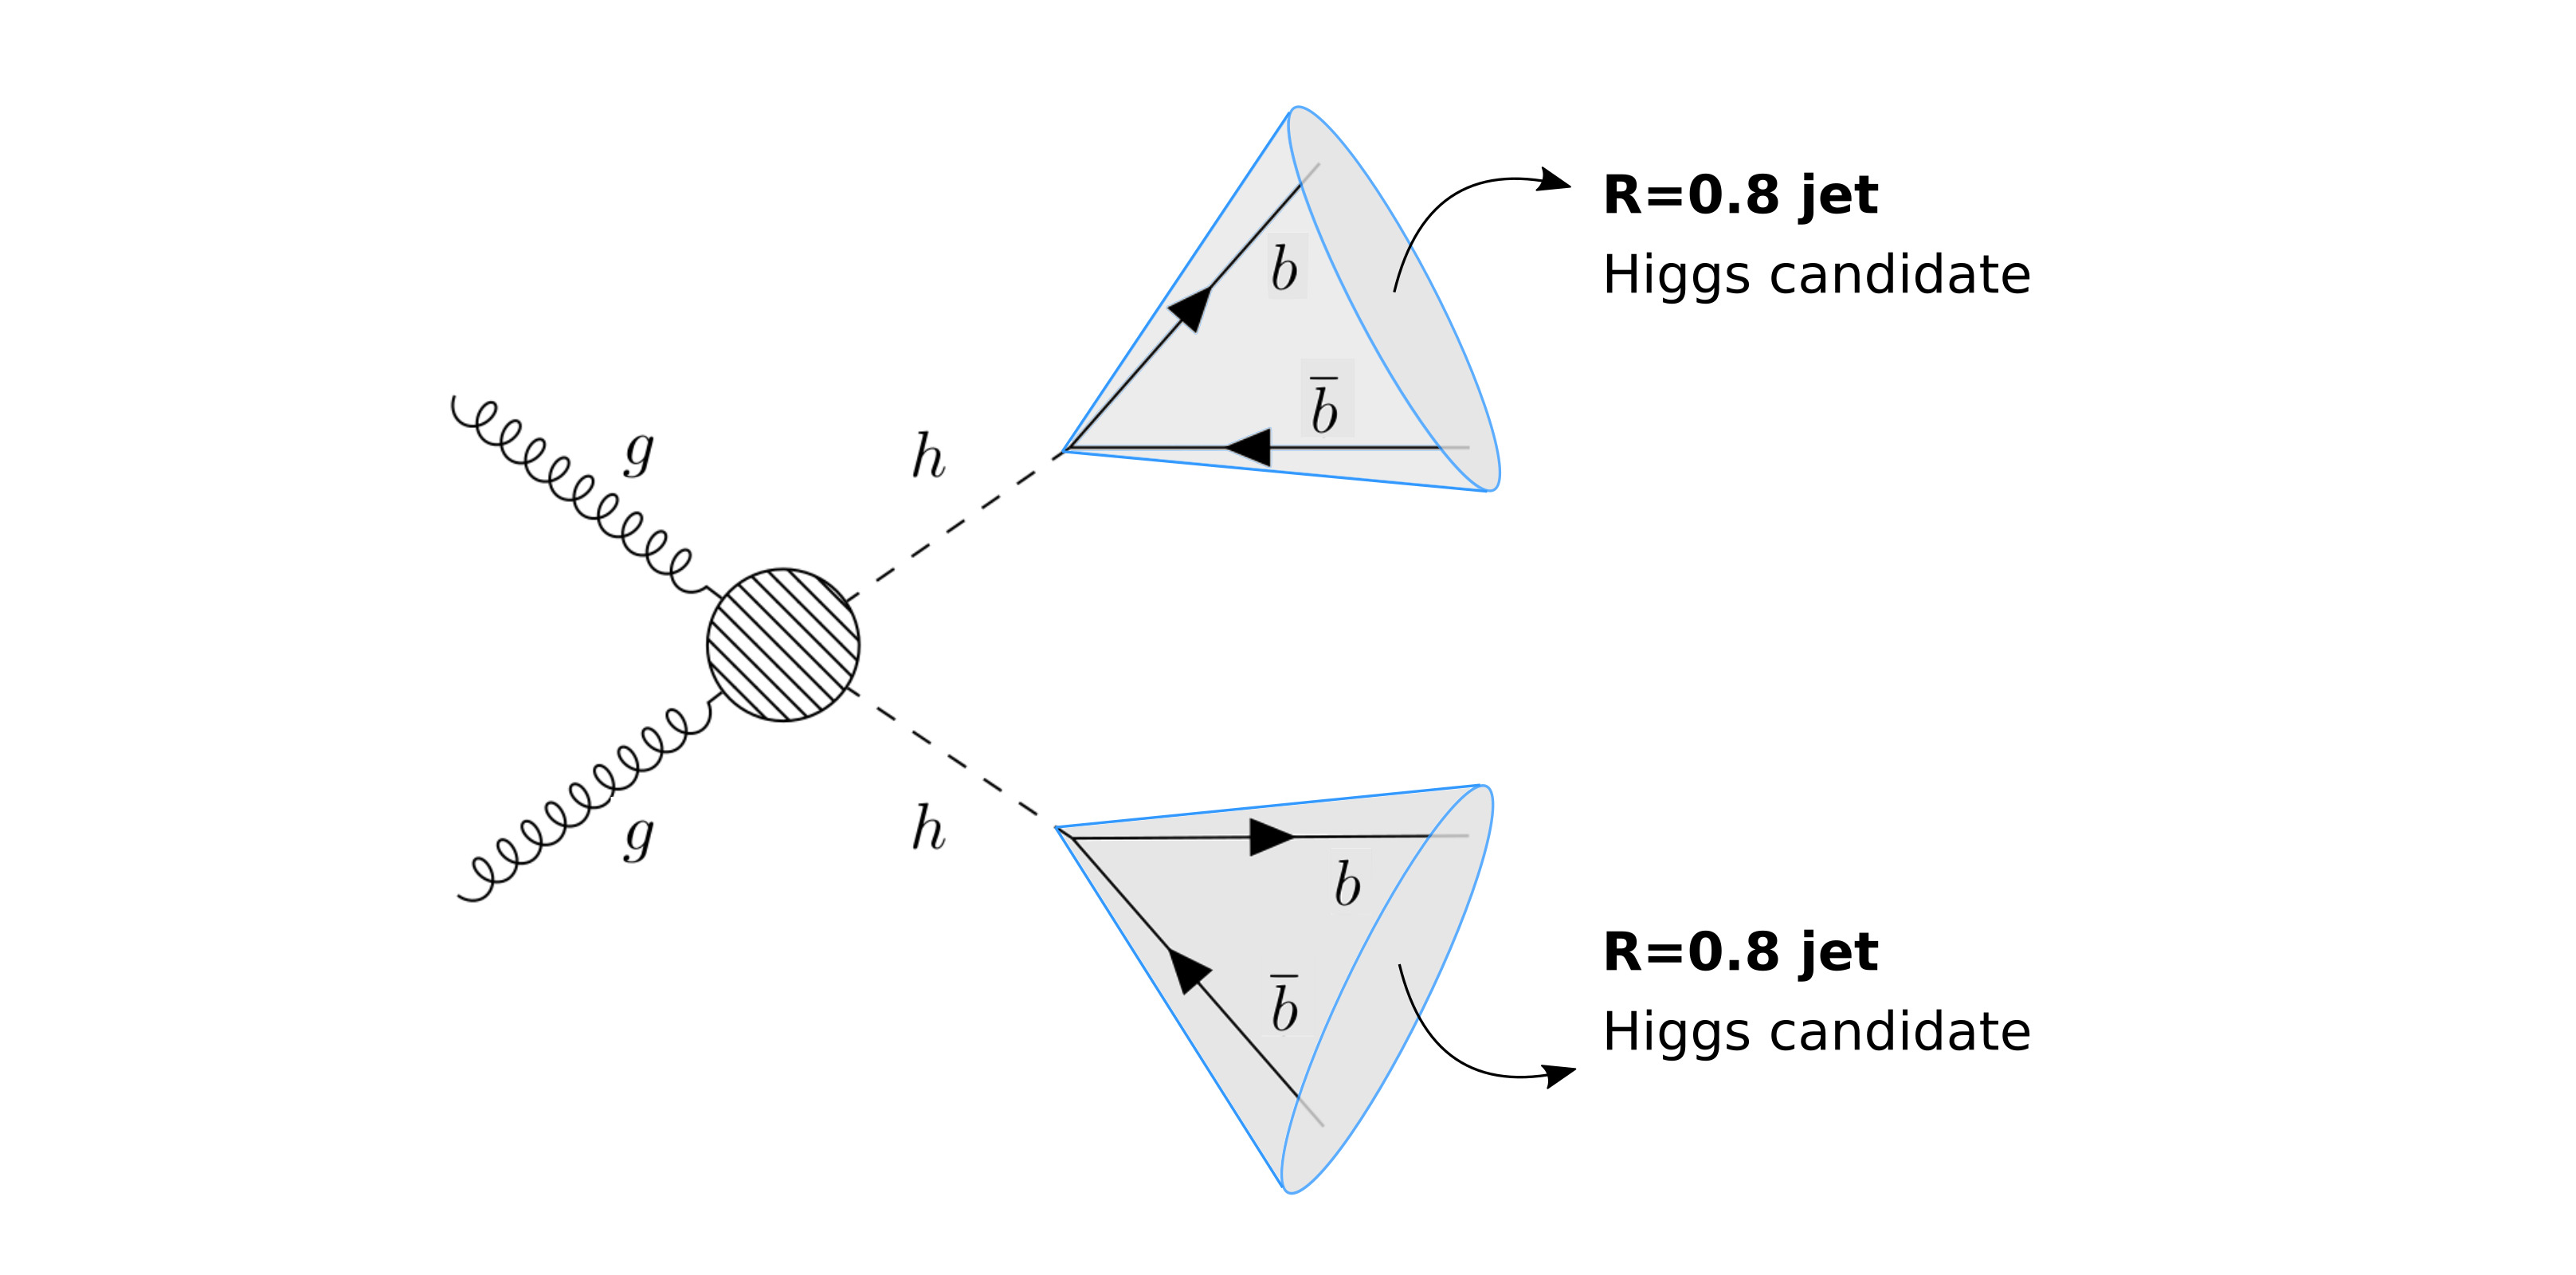
\includegraphics[trim={4.5cm .5cm 1cm .5cm},clip,width=1.2\linewidth]{./images/boosted1.png}
	\label{fig:boosted}
	\caption{oi}
\end{figure}

The events are reconstructed using particle flow (or calorimeter) jets with $R=0.8$ clustered with the anti-$k_T$ algorithm. The events are required to have at least two jets. Each jet is required to have two subjets, both b-tagged. In addition, both jets are required to have $p_T>200$ GeV. These cuts consist of the event pre-selection.

The b-tagging is implemented using truth level information. The b-tagging and mis tagging efficiencies are extracted from the FCC-hh detector default Delphes card, implemented by the FCC-hh study group.

The event selection is described in the following paragraphs. The value of the cuts follow from a scan over all the possible cut values. We choose the cut value that maximizes the significance, $S/\sqrt{B}$. 

We require
\begin{equation}
	p_T(h_1)>300~\text{GeV}, \quad p_T(hh)>100 ~\text{GeV}
\end{equation}
where $p_T(h_1)$, $p_T(hh)$ are the transverse momentums of the leading Higgs candidate and of the pair of Higgs candidates.
These cuts help suppress multijet background whose $p_T$ distributions fall more steeply than for the signal. A requirement on the maximum value of the N-subjetiness variable of the leading and subleading Higgs candidates, $\tau_{21}(h_1,h_2)]$ to further reject jets that are not consistent with a two-prong substructure:
\begin{equation}
	\tau_{21}(h_1,h_2)<0.4.
\end{equation}
These cuts work as a Higgs tagging criteria.

\begin{figure}[h]
	\centering
	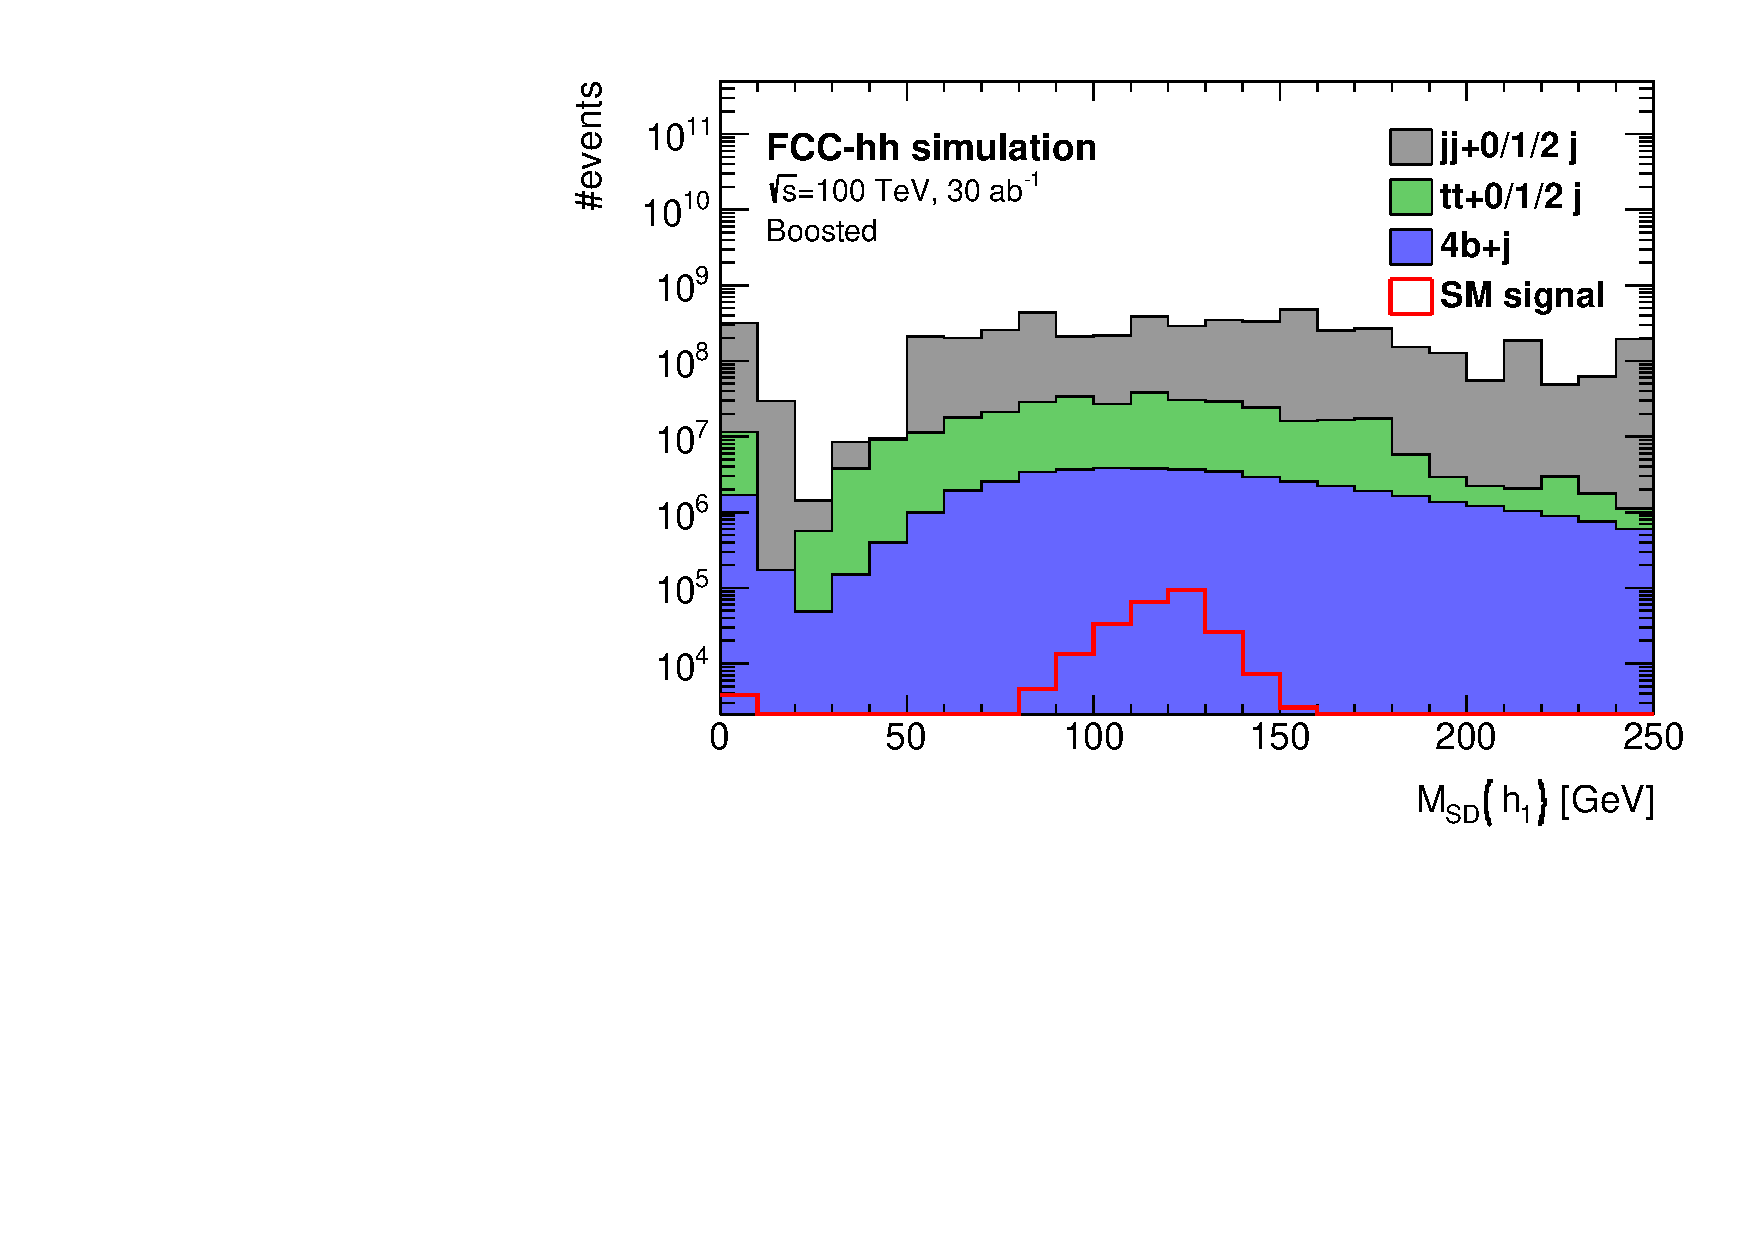
\includegraphics[width=\linewidth]{./images/hist_h1_softdrop_M_stack.pdf}
	\label{fig:stack}
	\caption{oi}
\end{figure}



%%%%%%%%%%%%%%%%%%%%%%%%%%%%%%%%%%%%%%%%%%%%%%%%%%%%%%%%%%%%%%%%%%%%%%
% RESULTS
%%%%%%%%%%%%%%%%%%%%%%%%%%%%%%%%%%%%%%%%%%%%%%%%%%%%%%%%%%%%%%%%%%%%%%
%%%%%%%%%%%%%%%%%%%%%%%%%%%%%%%%%%%%%%%%%%%%%%%%%%%%%%%%%%%%%%%%%%%%%%
%     File: ExtendedAbstract_resul.tex                               %
%     Tex Master: ExtendedAbstract.tex                               %
%                                                                    %
%     Author: Andre Calado Marta                                     %
%     Last modified : 27 Dez 2011                                    %
%%%%%%%%%%%%%%%%%%%%%%%%%%%%%%%%%%%%%%%%%%%%%%%%%%%%%%%%%%%%%%%%%%%%%%
% Results
% Results should be clear and concise.
% Discussion
% This should explore the significance of the results of the work, not
% repeat them. A combined Results and Discussion section is often
% appropriate. Avoid extensive citations and discussion of published
% literature.
%%%%%%%%%%%%%%%%%%%%%%%%%%%%%%%%%%%%%%%%%%%%%%%%%%%%%%%%%%%%%%%%%%%%%%

\section{Results}
\label{sec:resul}

%- Cutflow table \\
%- ...

The analyses described in section \ref{sec:imple} was developed and optimized using samples simulated with the default FCC-hh detector implementation. The results are reported in terms of the significance, $S/\sqrt{B}$, that was achieved (section \ref{sec:results_FCC}). The same analysis is applied to the different detector configurations (describe in section \ref{sec:sim}) and the results compared in terms of significance and singnal efficiency (section \ref{sec:gran_studies}).  

\subsection{Higgs pair discovery potential at the FCC-hh}
\label{sec:results_FCC}

Considering the SM signal production the achieved significance is
\begin{equation}
	(S/\sqrt{B})_{SM}=8.8\pm 1.6~\text{(stat.)}~^{+4.4}_{-3.4}~\text{(sys.)}
\end{equation}
for an integrated luminosity of $30~\text{ab}^{-1}$. The value of the significance is above the observation threshold ($5\sigma$) which indicates that the full dataset that is expected to be accumulated in the FCC-hh should be enough to declare the observation (or to exclude) the production of Higgs pairs as predicted by the SM.

For the $1$ TeV DM mediator signal, the significance is $2.3\pm0.4~\text{(stat.)}~^{+1.2}_{-0.9}~\text{(sys.)}$ for $\mathcal{L}=30~\text{ab}^{-1}$ which make a challenging and probably inaccessible benchmark. For the 2HDM signal the achieved significance is 
\begin{equation}
	(S/\sqrt{B})_{2HDM}=16.9\pm 3.0~\text{(stat.)}~^{+8.5}_{-6.6}~\text{(sys.)}
\end{equation}
for $\mathcal{L}=30~\text{ab}^{-1}$, making it a very interesting benchmark model from the point of view of enhancing Higgs pair production with respect to the SM. 

The signal efficiency is higher for both BSM models than for the SM because the masses of the new heavy resonances were chosen to be large ($O(1 ~\text{TeV})$) to produce highly boosted Higgs pairs. For the SM the efficiency is $0.446\%$. It increases to $0.487\%$ for the DM mediator model and to $1.666\%$ for the 2HDM. 

\subsection{Granularity studies for future colliders}
\label{sec:gran_studies}

Figure \ref{fig:eff_gran} shows the signal efficiency (in percentage) as a function of the detector configuration. The left most point corresponds to the ATLAS detector and the right most point to the FCC-hh detector with a granularity twice as good in $\eta$ and $\phi$ (configuration 5 in table \ref{table:Gran}). The points in between are ordered by increasing granularity of the HCAL. All other plots that show some quantity as a function of detector configuration follow the same convention. For all signal models, the efficiency increases as the granularity of the HCAL increases. It increases by approximately $30\%$ from the first to the last points.

Figures \ref{fig:SSB_gran} and \ref{fig:SSB_gran_2HDM} show the significance ($S/\sqrt{B}$) as a function of the detector configuration for the SM signal model and for the 2HDM, respectively. Triangular markers represent analysis that were performed using pure HCAL jets while square markers represent analysis performed using energy flow jets. 

Although the uncertainties . For energy flow jets the change in significance is very mild. It varies by approximately $30\%$ between the first and last points, for both signal models. It becomes more pronounced when using pure calorimeter jets. It varies by approximately $70\%~(55\%)$ between the first and last points for the SM (2HDM) signal. However, when using calorimeter jets, the achieved significance is always smaller (for the same detector configuration) because we are not using information from the tracking system. This is verified for both the SM and 2HDM signals. These results indicate that when using energy flow jets the tracking system is dominating the jet reconstruction.

\begin{figure}[h]
	\centering
	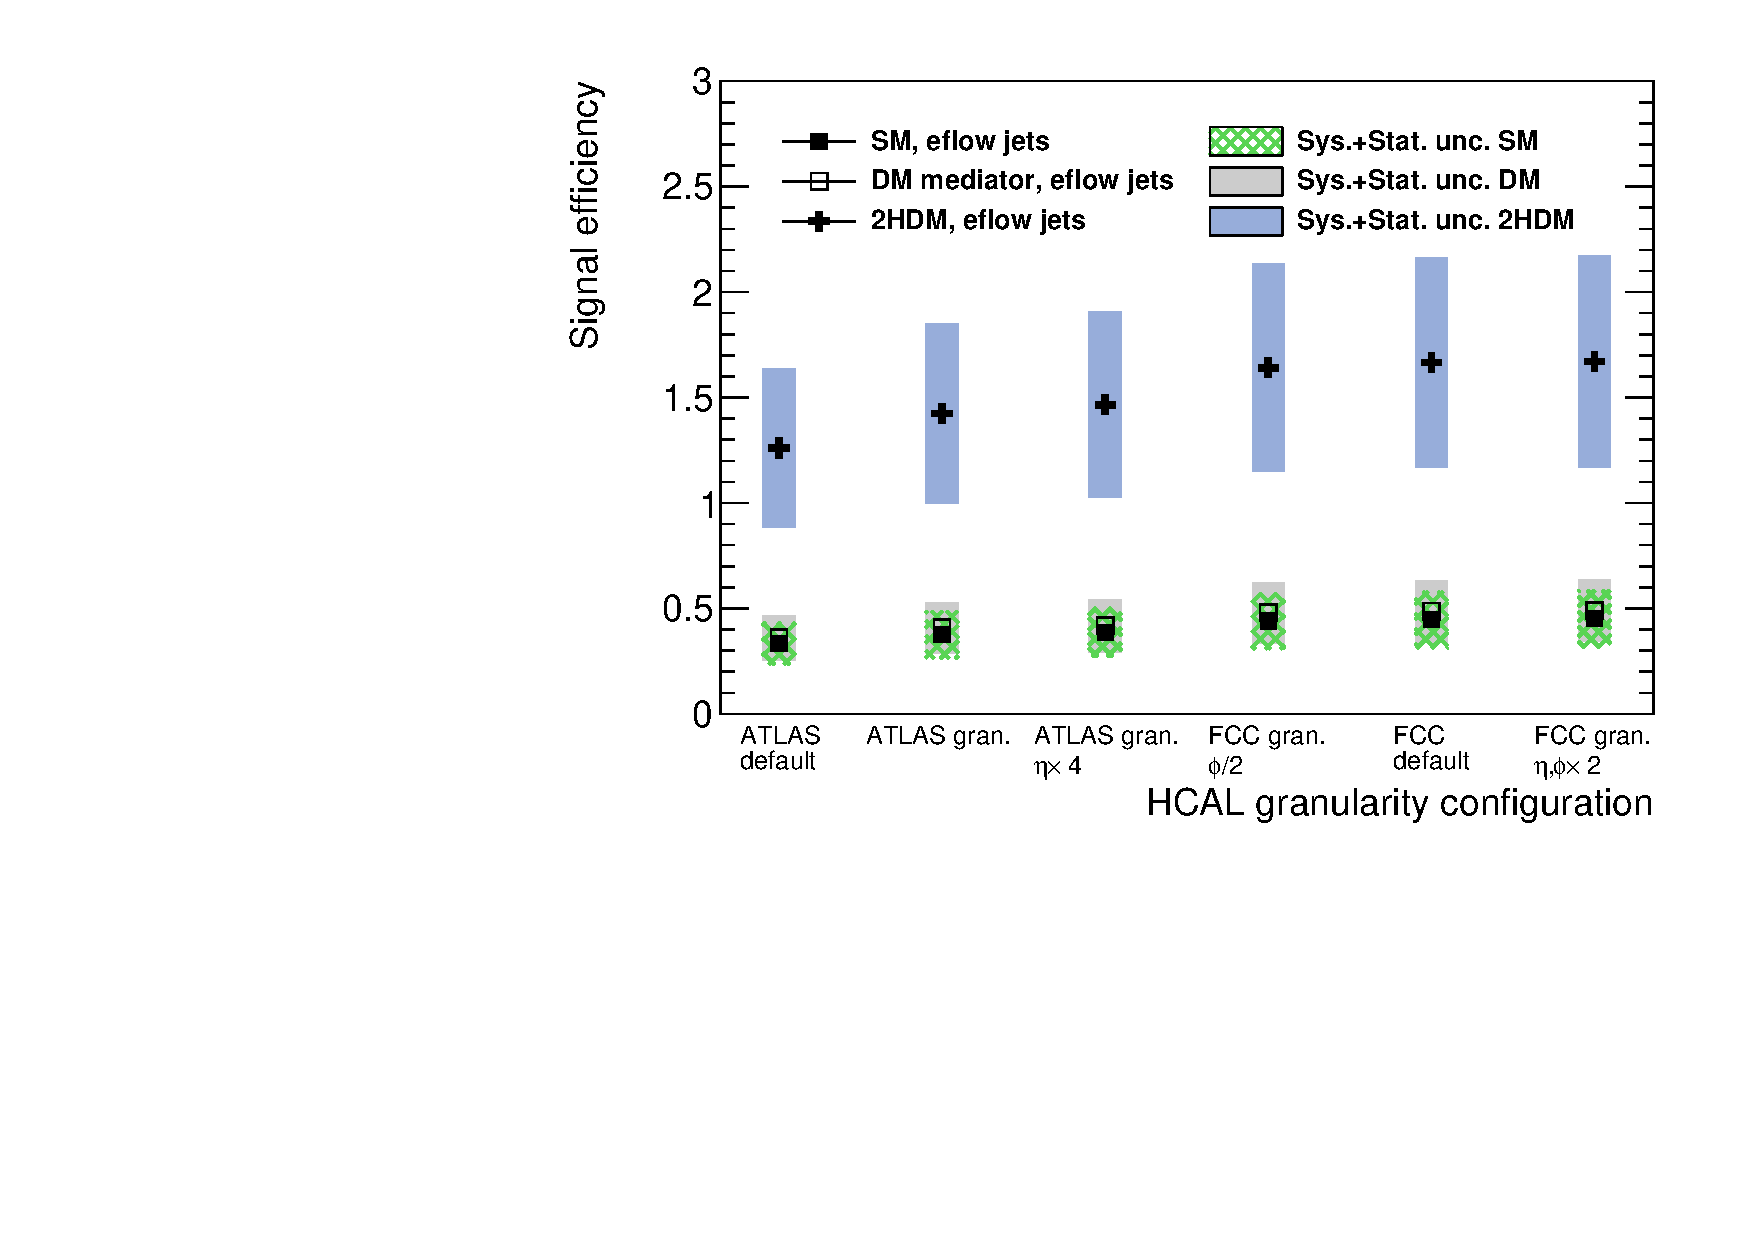
\includegraphics[width=\linewidth]{./images/EffvsGran_PFjets_Opt.pdf}
	\caption{Signal efficiency in percentage as a function of the detector configuration. The statistical error bars are drawn but are smaller than the markers.}
	\label{fig:eff_gran}
\end{figure}

\begin{figure}[h]
	\centering
	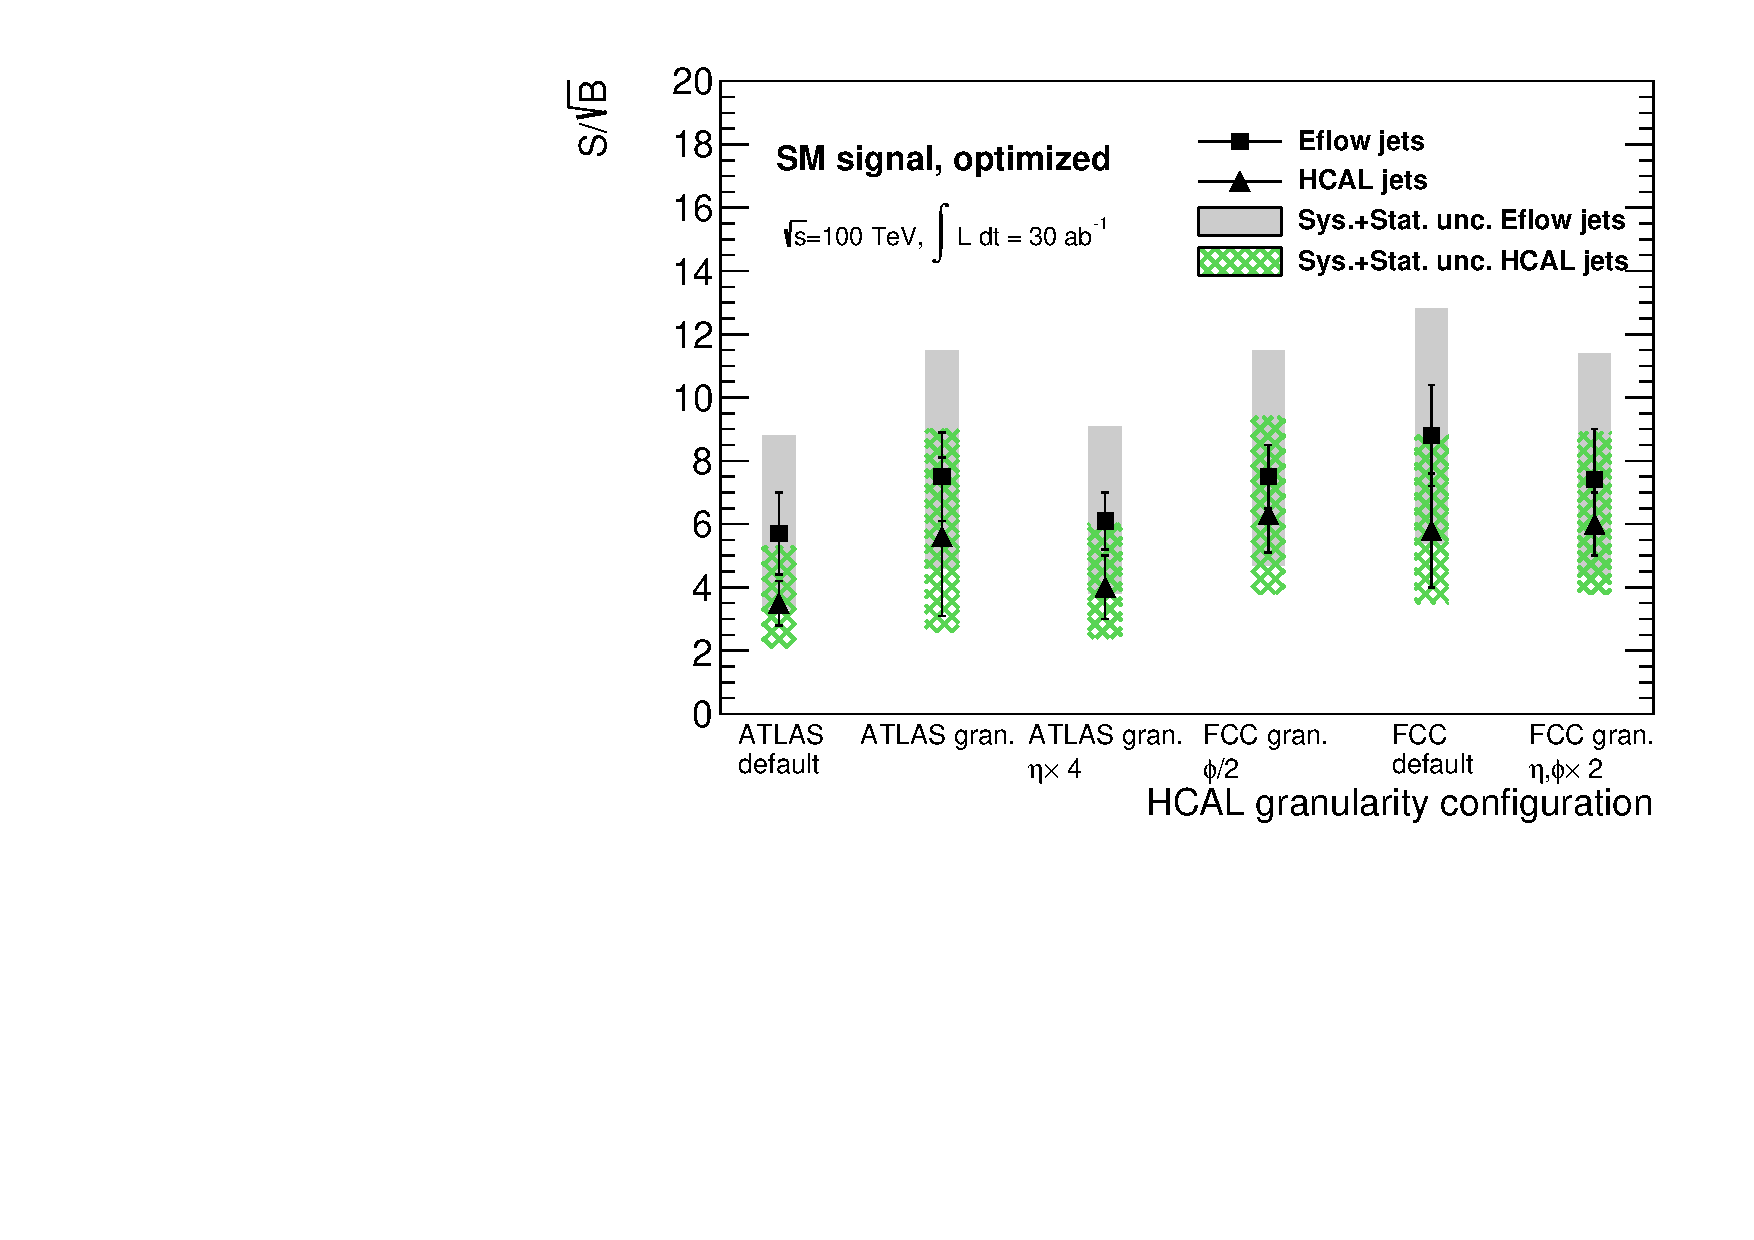
\includegraphics[width=\linewidth]{./images/SSBvsGran_SM_Opt.pdf}
	\caption{$S/\sqrt{B}$ as a function of the detector configuration for the SM signal model. The square (triangular) markers refer to values obtained using particle flow (calorimeter) jets.}
	\label{fig:SSB_gran}
\end{figure}

\begin{figure}[h]
	\centering
	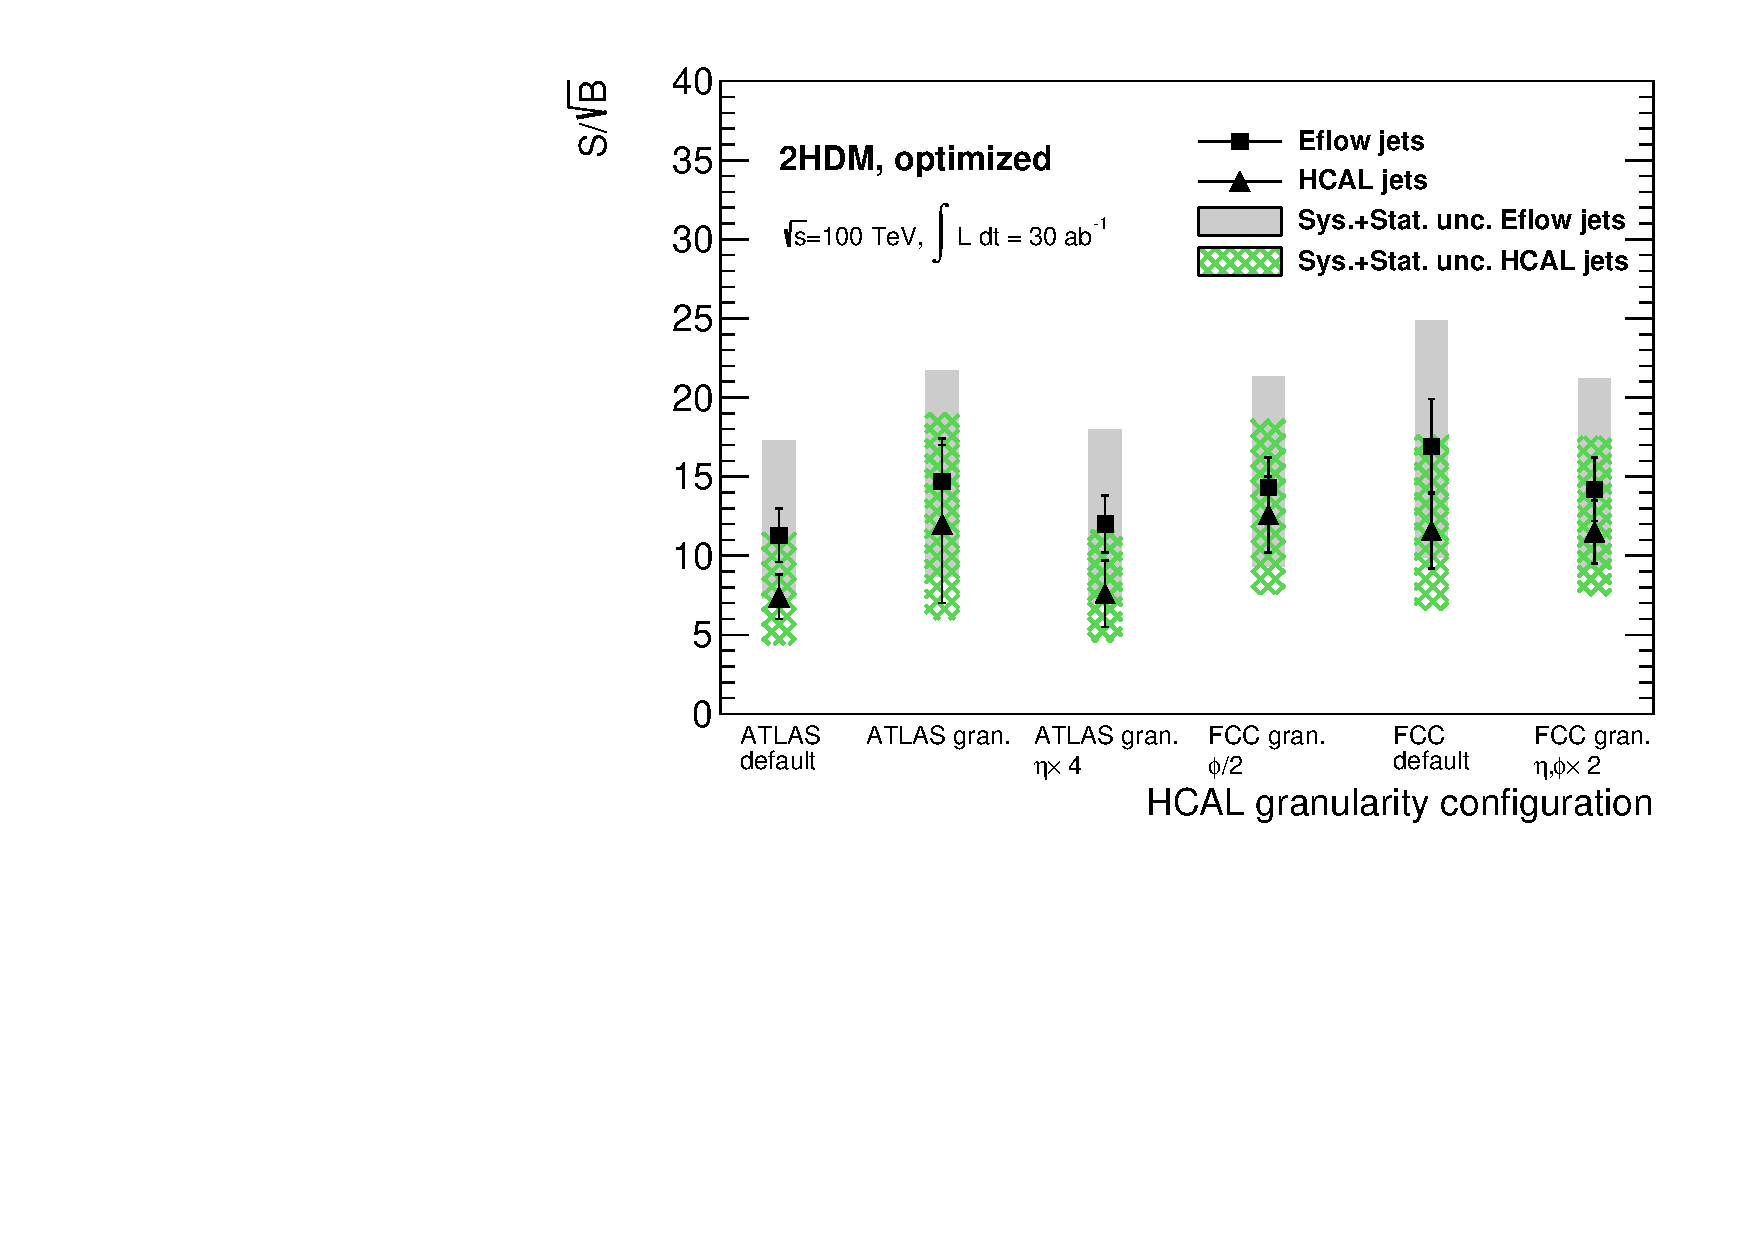
\includegraphics[width=\linewidth]{./images/SSBvsGran_2HDM_Opt.pdf}
	\caption{$S/\sqrt{B}$ as a function of the detector configuration for the 2HDM signal model. The square (triangular) markers refer to values obtained using particle flow (calorimeter) jets.}
	\label{fig:SSB_gran_2HDM}
\end{figure}



%%%%%%%%%%%%%%%%%%%%%%%%%%%%%%%%%%%%%%%%%%%%%%%%%%%%%%%%%%%%%%%%%%%%%%
% CONCLUSIONS
%%%%%%%%%%%%%%%%%%%%%%%%%%%%%%%%%%%%%%%%%%%%%%%%%%%%%%%%%%%%%%%%%%%%%%
%%%%%%%%%%%%%%%%%%%%%%%%%%%%%%%%%%%%%%%%%%%%%%%%%%%%%%%%%%%%%%%%%%%%%%
%     File: ExtendedAbstract_concl.tex                               %
%     Tex Master: ExtendedAbstract.tex                               %
%                                                                    %
%     Author: Andre Calado Marta                                     %
%     Last modified : 27 Dez 2011                                    %
%%%%%%%%%%%%%%%%%%%%%%%%%%%%%%%%%%%%%%%%%%%%%%%%%%%%%%%%%%%%%%%%%%%%%%
% The main conclusions of the study presented in short form.
%%%%%%%%%%%%%%%%%%%%%%%%%%%%%%%%%%%%%%%%%%%%%%%%%%%%%%%%%%%%%%%%%%%%%%

\section{Conclusions}
\label{sec:concl}

This article presented a feasibility study targeting the search for Higgs pair production in the $pp\rightarrow hh\rightarrow b\overline{b}b\overline{b}$ channel at a center of mass energy of $\sqrt{s}=100$ TeV. The analysis is based on rectangular cut on kinematic and substructure variables and targets the boosted event topology. The main backgrounds are QCD multijet and $t\overline{t}$ production. The impact of the granularity of the hadronic calorimeter in the achieve significance was studied. 

Three signal model are investigated: SM, $1$ TeV dark matter spin-$0$ mediator and CP-conserving type II 2HDM with $m_H=900$ GeV. Due to the small cross section, the DM mediator model originates a significance of the order of $2$, making it a very challenging and probably unaccessible background. 

For the FCC-hh, the significances achieved for the SM and 2HDM signal modes were $(S/\sqrt{B})_{SM}=8.8\pm 1.6~\text{(stat.)}~^{+4.4}_{-3.4}~\text{(sys.)}$ and $(S/\sqrt{B})_{2HDM}=16.9\pm 3.0~\text{(stat.)}~^{+8.5}_{-6.6}~\text{(sys.)}$, respectively, for an integrated luminosity of $\mathcal{L}=30~\text{ab}^{-1}$. These values are above the $5\sigma$ threshold which indicates that the total dataset that is expected to be collected at the FCC-hh should be enough to observe (or exclude) the production of Higgs pairs in these model.

For particle flow jets, the efficiency of the signal increases as the granularity of the HCAL increases. It varies by approximately $30\%$ between the ATLAS detector configuration and the detector configuration with twice the granularity of the FCC baseline detector in $\eta$a and $\phi$. It is harder to discern such a clear tendency for the significance because the statistical fluctuations are large which is due to the large statistical weight of the multijet background. Nonetheless, for particle flow (calorimeter) jets, the significance varies by approximately $30\%~(70\%)$, for the SM signal model. 

As future work, performing similar studies using different benchmark processes and full detector simulation seems to be of the utmost importance in order to optimize the designe of future detectors.



%%%%%%%%%%%%%%%%%%%%%%%%%%%%%%%%%%%%%%%%%%%%%%%%%%%%%%%%%%%%%%%%%%%%%%
% ACKNOWLEDGMENTS
%%%%%%%%%%%%%%%%%%%%%%%%%%%%%%%%%%%%%%%%%%%%%%%%%%%%%%%%%%%%%%%%%%%%%%
%%%%%%%%%%%%%%%%%%%%%%%%%%%%%%%%%%%%%%%%%%%%%%%%%%%%%%%%%%%%%%%%%%%%%%
%     File: ExtendedAbstract_ackno.tex                               %
%     Tex Master: ExtendedAbstract.tex                               %
%                                                                    %
%     Author: Andre Calado Marta                                     %
%     Last modified : 27 Dez 2011                                    %
%%%%%%%%%%%%%%%%%%%%%%%%%%%%%%%%%%%%%%%%%%%%%%%%%%%%%%%%%%%%%%%%%%%%%%
% Acknowledge persons and institutions that supported this work.
%%%%%%%%%%%%%%%%%%%%%%%%%%%%%%%%%%%%%%%%%%%%%%%%%%%%%%%%%%%%%%%%%%%%%%

\section*{Acknowledgements}

The author would like to thank Ricardo Gon\c calo for supervising this work, contributing with invaluable scientific advise and ultimately making it possible. The author would also like to acknowledge the support of the Funda\c c\~ao para a Ci\^encia e Tecnologia through the CERN/FIS-PAR/0008/2017 grant.


%%%%%%%%%%%%%%%%%%%%%%%%%%%%%%%%%%%%%%%%%%%%%%%%%%%%%%%%%%%%%%%%%%%%%%
% REFERENCES
%%%%%%%%%%%%%%%%%%%%%%%%%%%%%%%%%%%%%%%%%%%%%%%%%%%%%%%%%%%%%%%%%%%%%%

% Produces the bibliography section when processed by BibTeX
%
% Bibliography style
% > entries ordered alphabetically
%\bibliographystyle{plain}
% > unsorted with entries appearing in the order in which the citations appear.
\bibliographystyle{elsarticle-num}
% > entries ordered alphabetically, with first names and names of journals and months abbreviated
%\bibliographystyle{abbrvunsrtnat}
% > entries ordered alphabetically, with reference markers based on authors' initials and publication year
%\bibliographystyle{alpha}

% External bibliography database file in the BibTeX format (ExtendedAbstract_ref_db.bib)
\bibliography{ExtendedAbstract_ref_db}

%%%%%%%%%%%%%%%%%%%%%%%%%%%%%%%%%%%%%%%%%%%%%%%%%%%%%%%%%%%%%%%%%%%%%%
\end{document}
%%%%%%%%%%%%%%%%%%%%%%%%%%%%%%%%%%%%%%%%%%%%%%%%%%%%%%%%%%%%%%%%%%%%%%

